\documentclass[compress,11pt]{beamer}
\usetheme{Ilmenau}
%\usecolortheme{beaver}
%\beamertemplatenavigationsymbolsempty
\usepackage{multimedia}
\usepackage[utf8]{inputenc}
\usepackage{amsmath}
\usepackage{amsfonts}
\usepackage{amssymb}
\usepackage{graphicx}
\usepackage{esvect}
%\author{}
\title{PP Gruppe 8}
%\setbeamercovered{transparent} 
%\setbeamertemplate{navigation symbols}{} 
%\logo{} 
%\institute{} 
%\date{} 
%\subject{} 
\usepackage{verbatim}
\begin{document}

\frame[c]{\titlepage}
\begin{frame}
\tableofcontents
\end{frame}


\section{Frequenzfilter}
\begin{frame}
	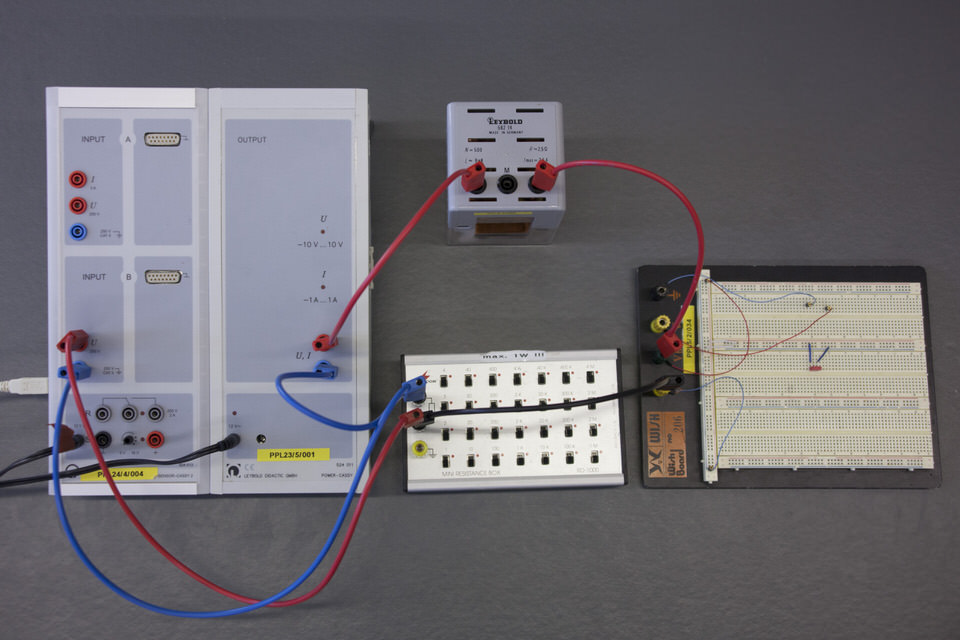
\includegraphics[width=\textwidth]{images/1/durchlassfilter}
\end{frame}

\begin{frame}
	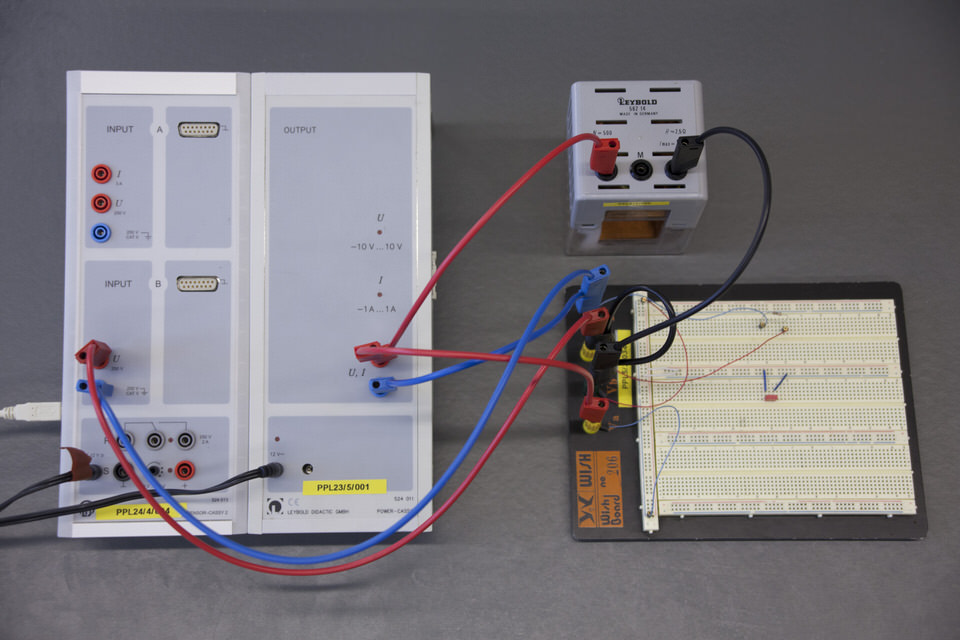
\includegraphics[width=\textwidth]{images/1/sperrfilter}
\end{frame}

\begin{frame}
	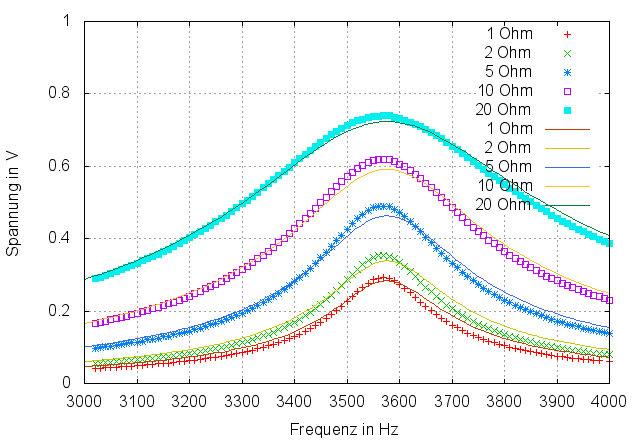
\includegraphics[width=\textwidth]{images/1/plot}
\end{frame}


\section{Michelson-Interferometer}
\begin{frame}
	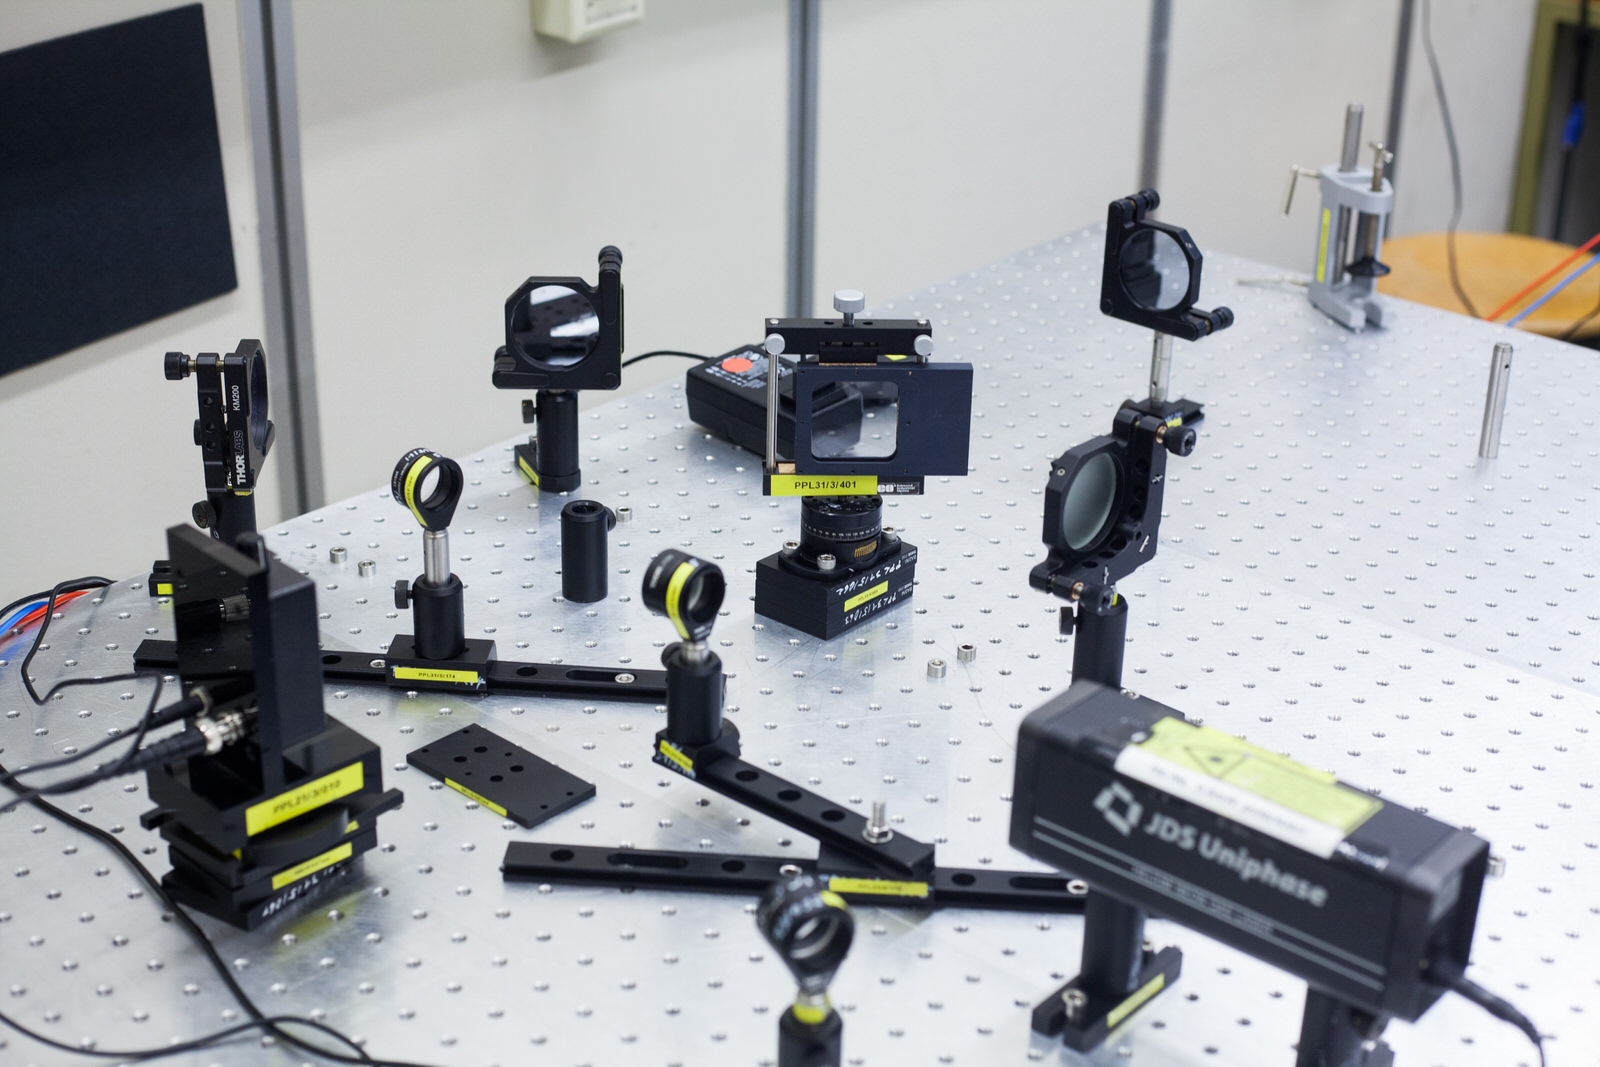
\includegraphics[width=\textwidth]{images/2/interferrometer-4}
\end{frame}

\begin{frame}
	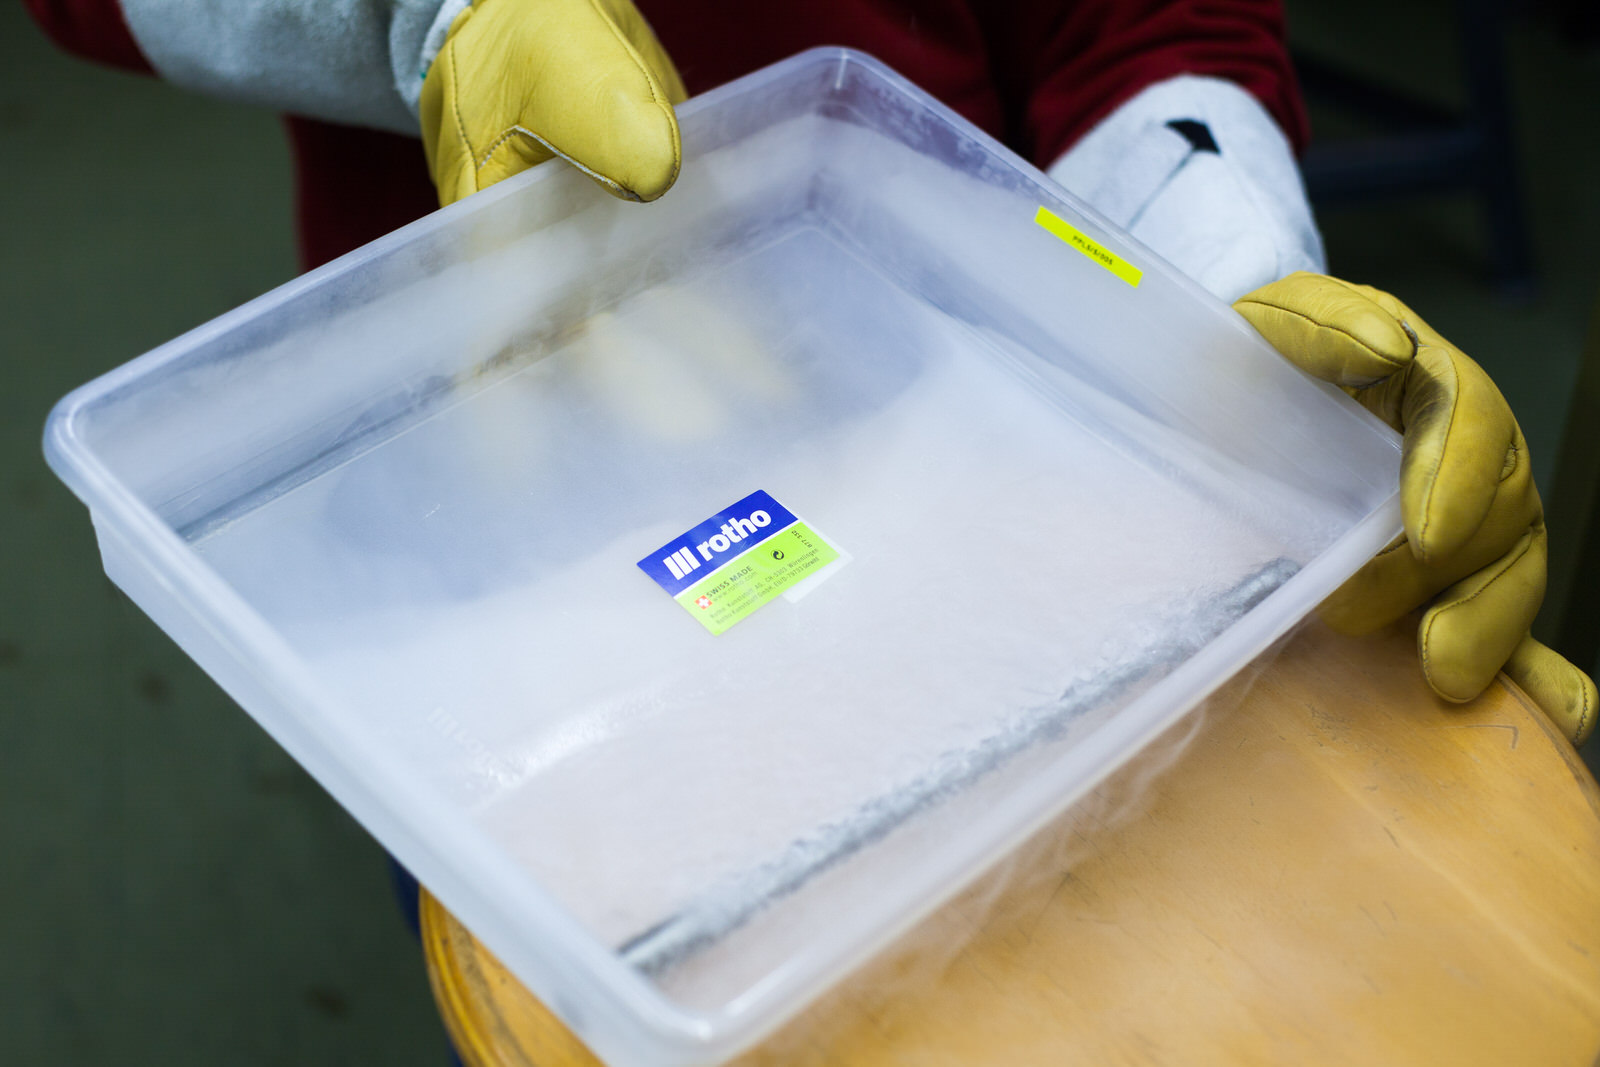
\includegraphics[width=\textwidth]{images/2/interferrometer-1}
\end{frame}

\begin{frame}
	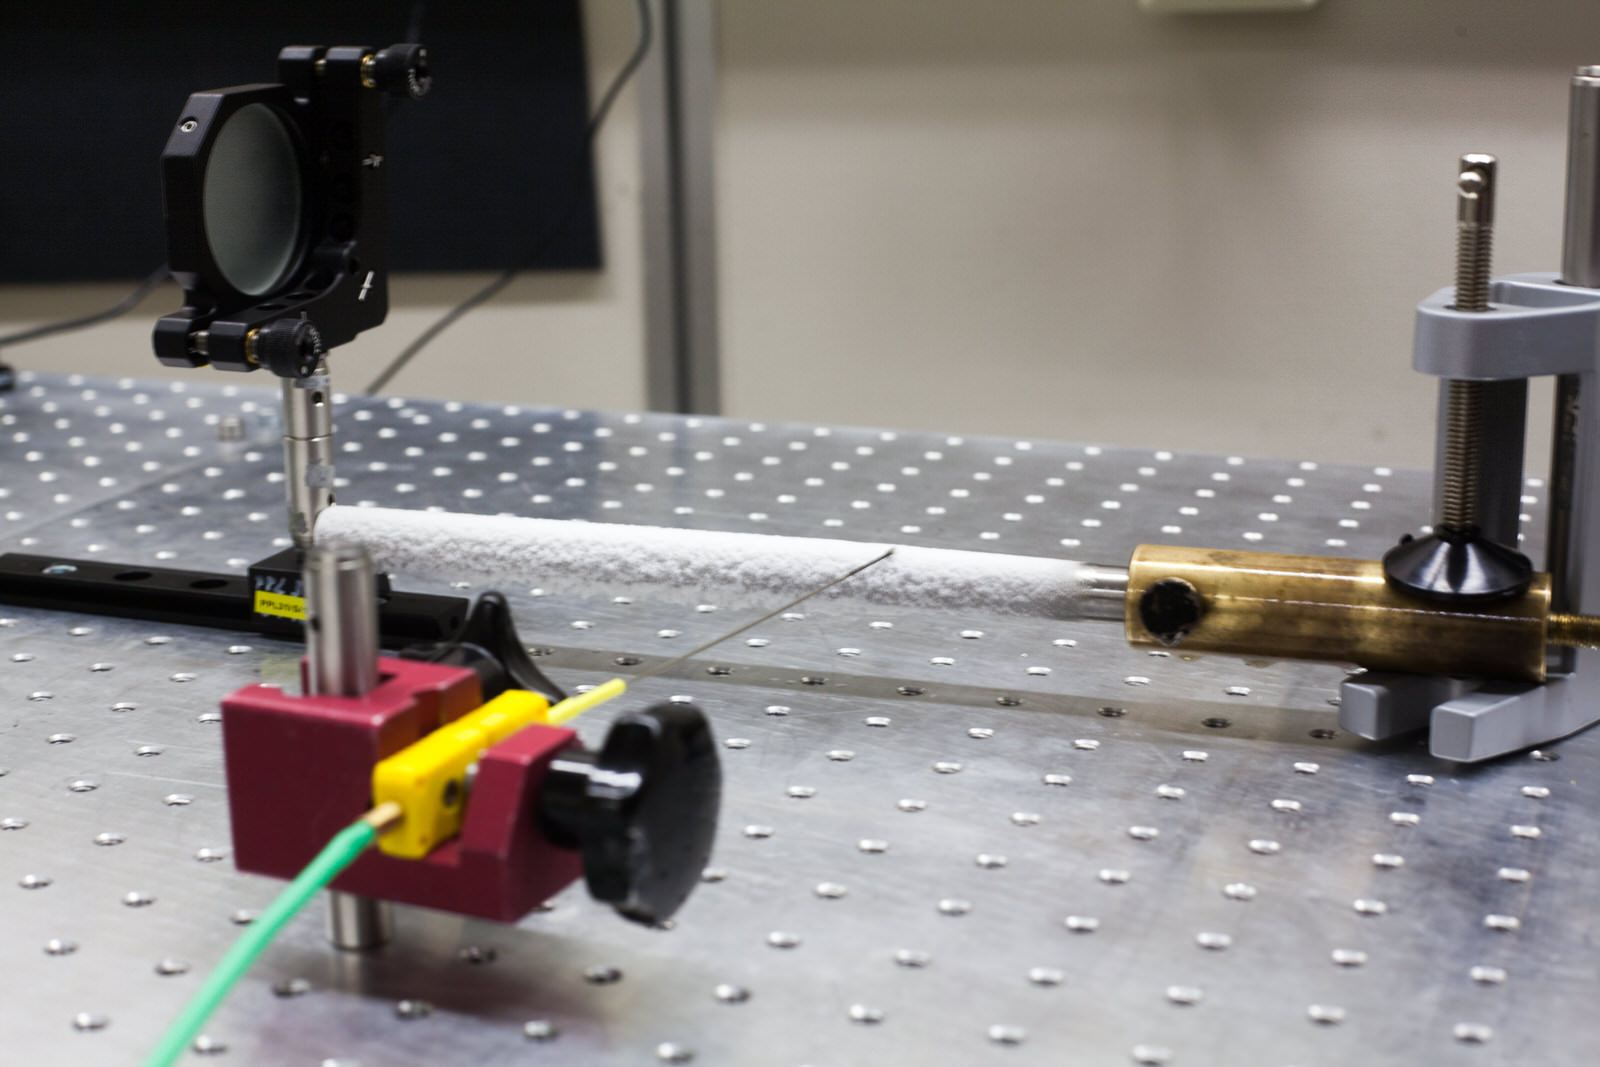
\includegraphics[width=\textwidth]{images/2/interferrometer-2}
\end{frame}

\begin{frame}
	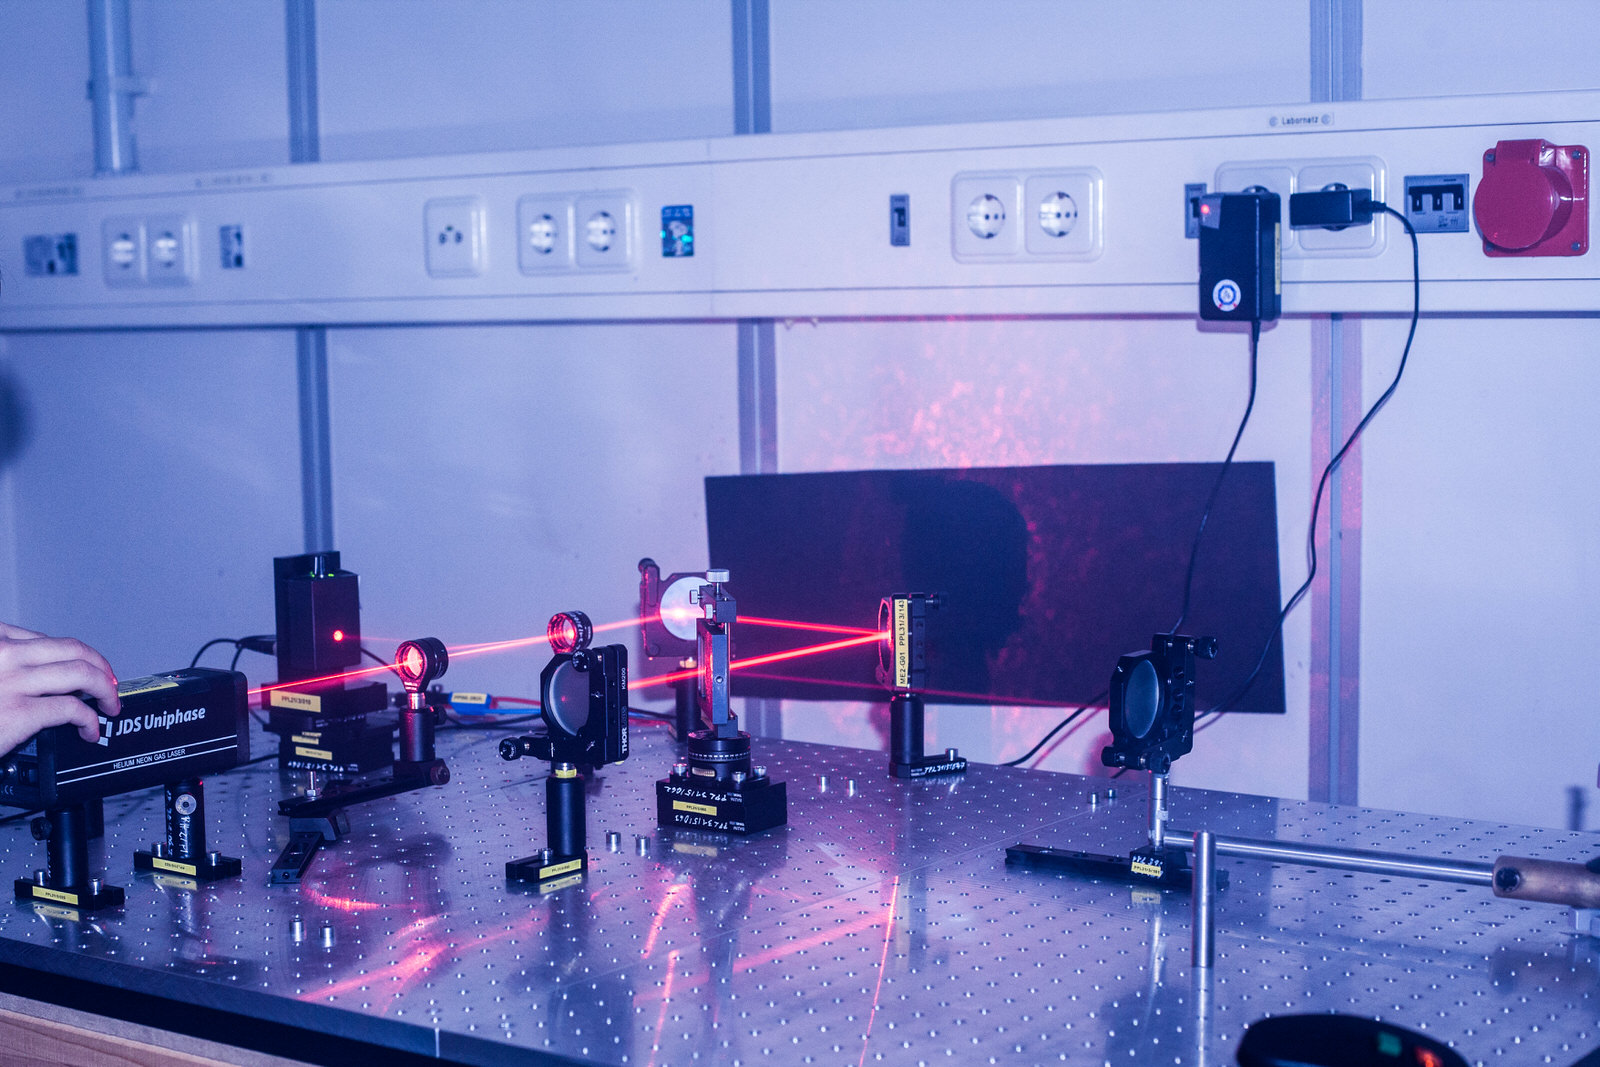
\includegraphics[width=\textwidth]{images/2/interferrometer-6}
\end{frame}


\section{Pitot}
\begin{frame}
	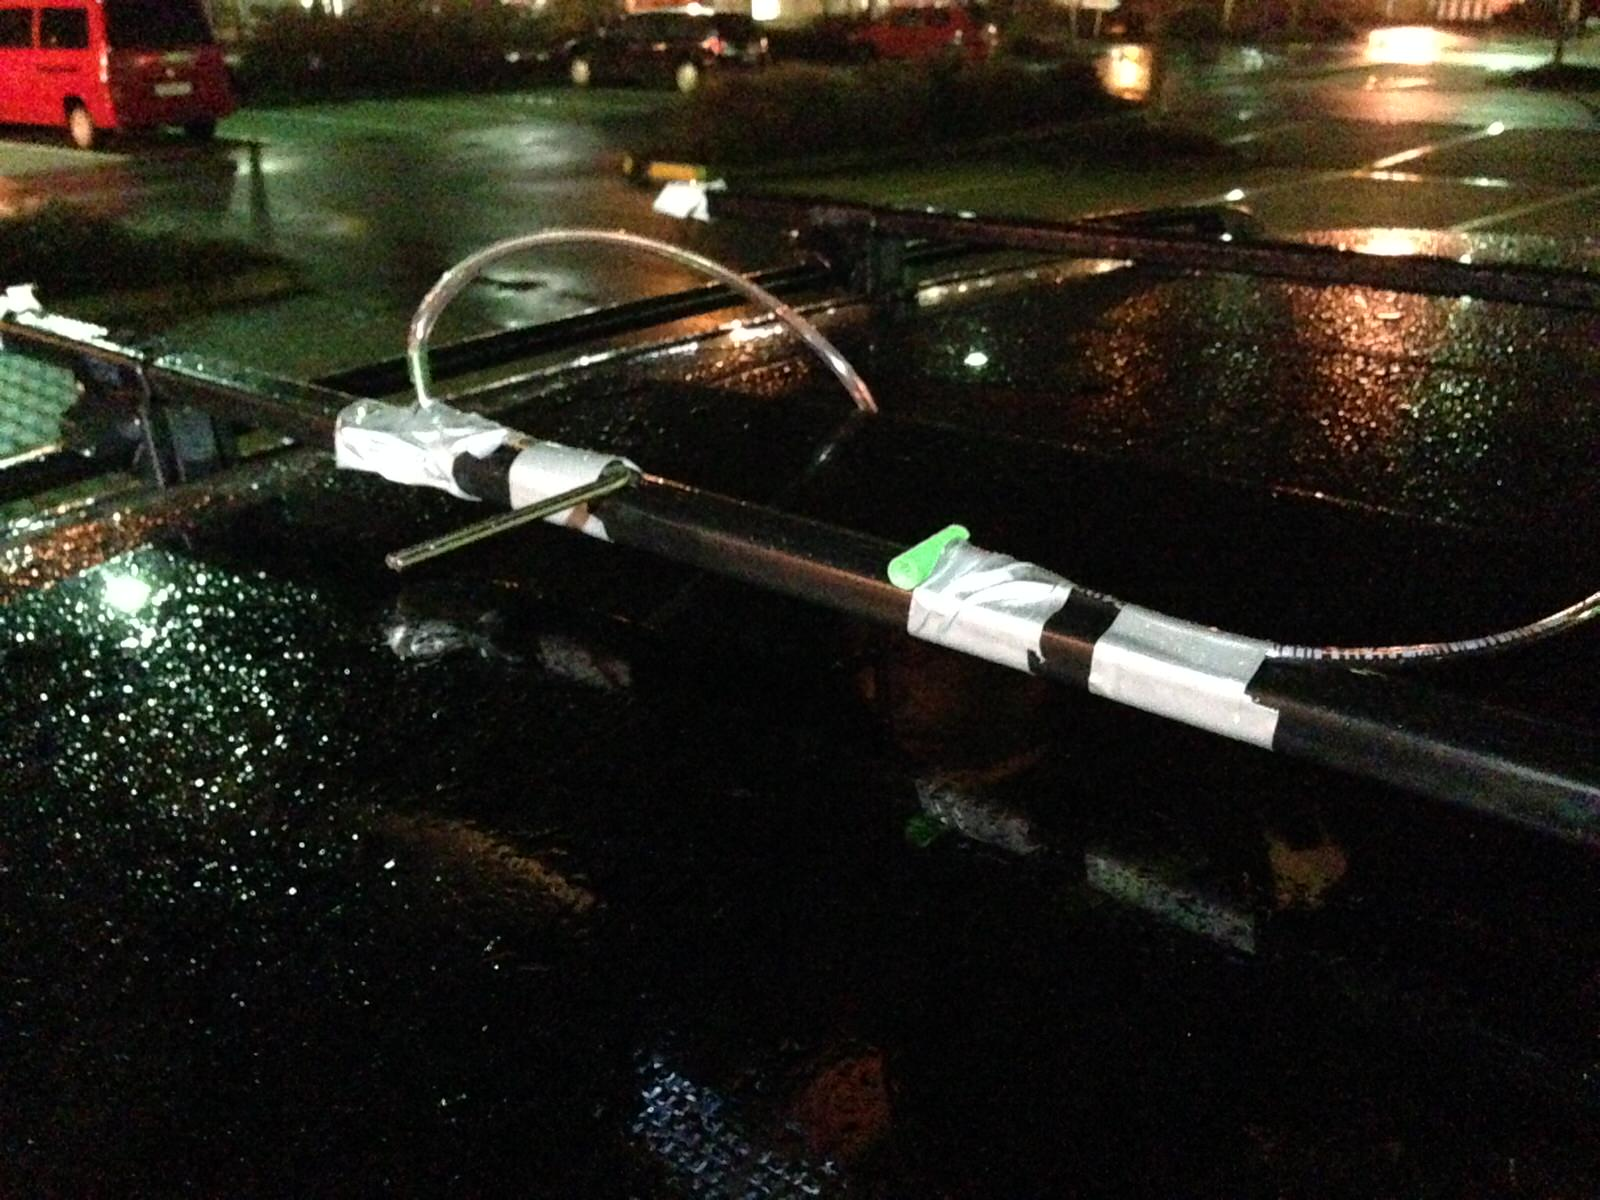
\includegraphics[width=\textwidth]{images/3/IMG_0004}
\end{frame}

\begin{frame}
	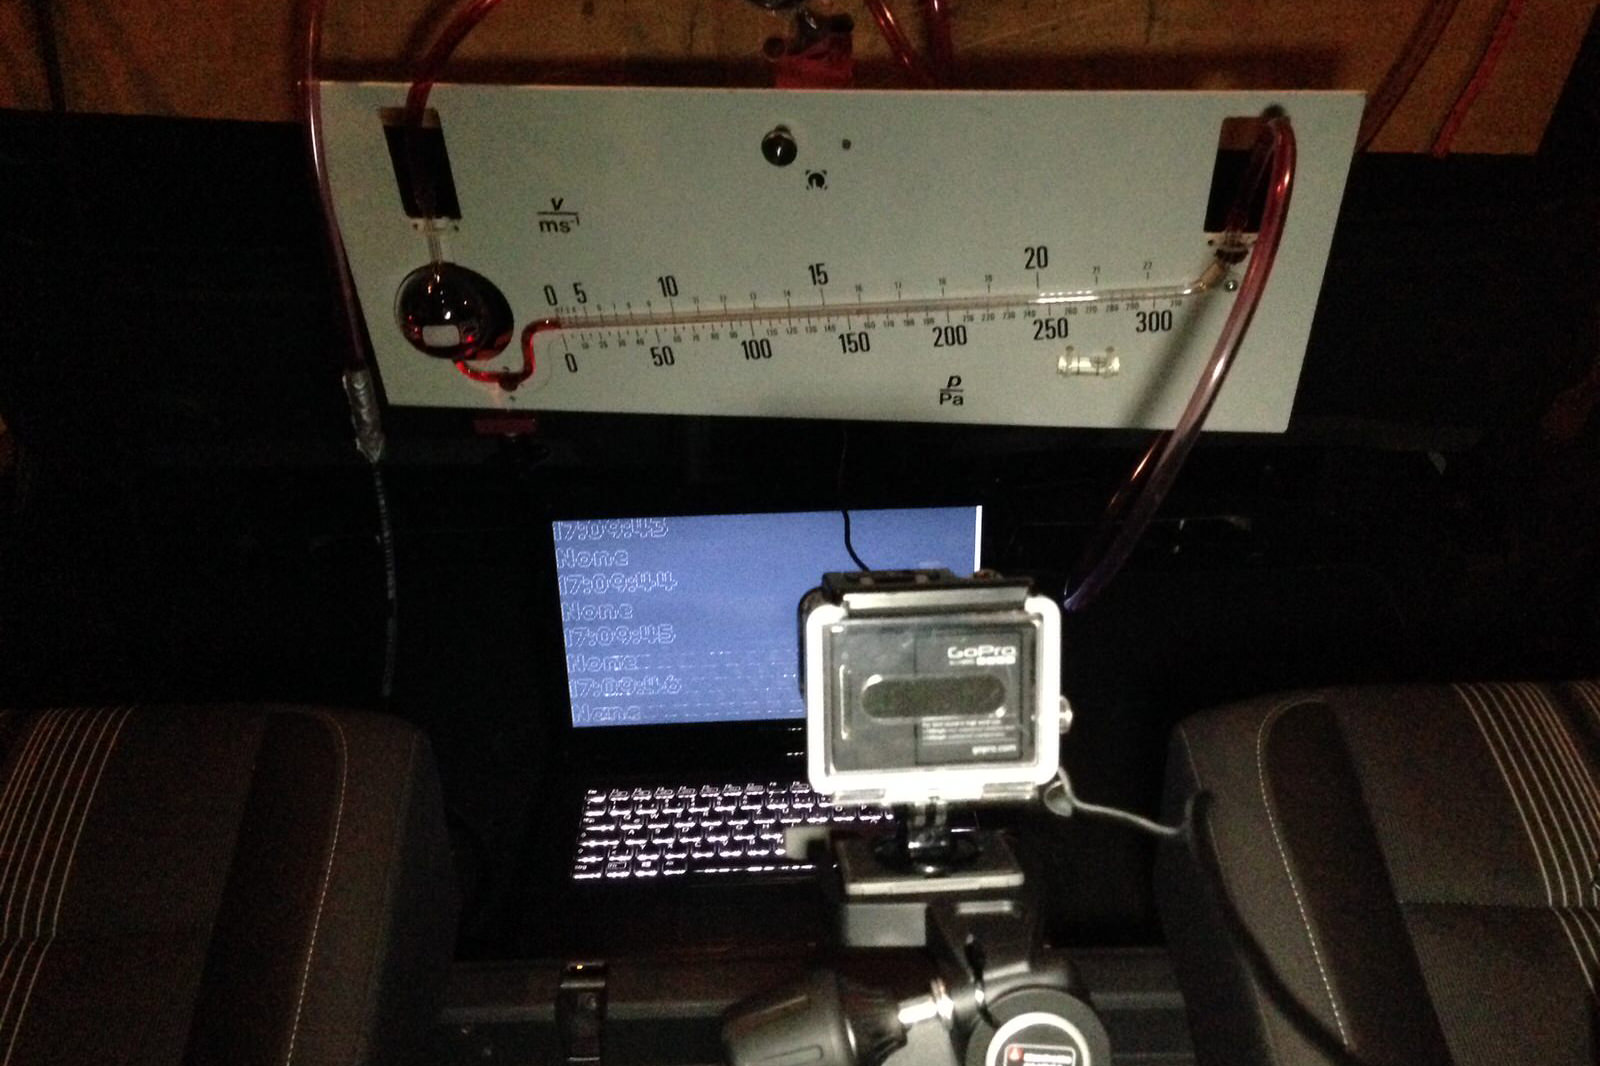
\includegraphics[width=\textwidth]{images/3/IMG_0007}
\end{frame}

\begin{frame}
	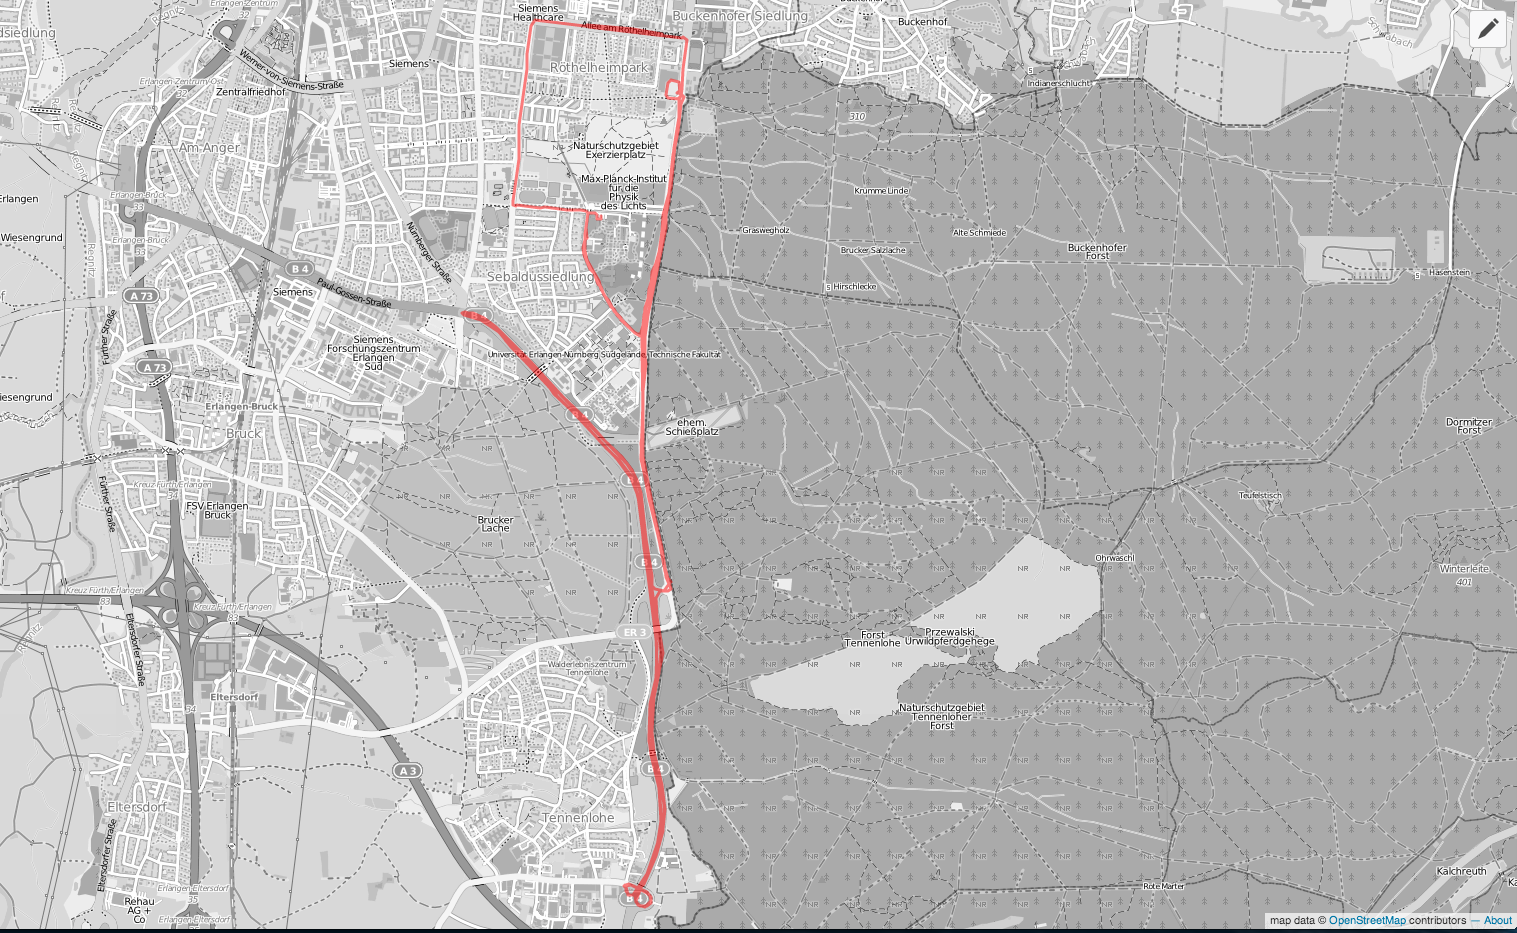
\includegraphics[width=\textwidth]{images/3/karte.png}
\end{frame}


\section{Doppelpendel}
\begin{frame}{Bestimmung der Bewegungsgleichungen mit Hilfe des Lagrangeformalismus}
	\begin{block}
		
		\begin{equation}
			\frac{d}{dt}\frac{\partial L}{\partial\dot{q_i}}-\frac{\partial L}{q_i} =0
		\label{lagrangegl}
		\end{equation}
		\begin{equation}
			 L=\sum_i E_{kin,i}-V_i=\sum_i \frac{m_i}{2}\cdot\dot{\vv{x_i}}^2 - m_i \cdot g \cdot z_i
		\end{equation}
	\end{block}
\end{frame}

%\begin{comment}
\begin{frame}

	\begin{minipage}{.48\textwidth}
	%\centering
	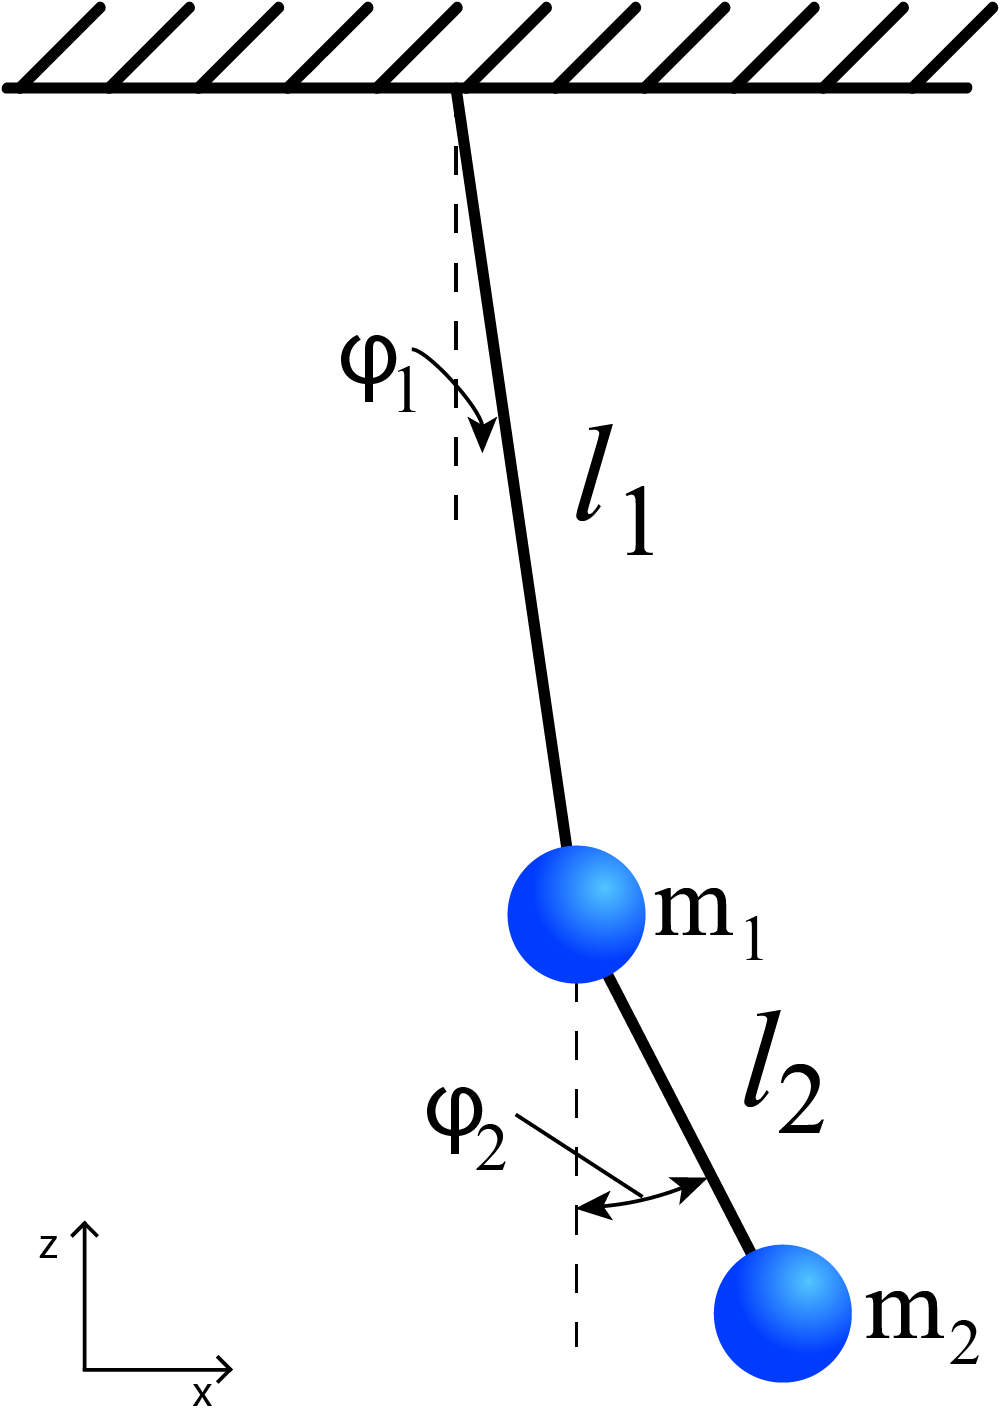
\includegraphics[width=\textwidth]{images/4/double-pendulum}
	\end{minipage}
	\begin{minipage}{.48\textwidth}
	\begin{block}{}
		\begin{equation}
			\vv{x_1}= l_1\cdot\begin{pmatrix}
			\sin \varphi_1 \\ -\cos \varphi_1
			\end{pmatrix}
		\end{equation}
		\begin{align}
			\vv{x_2}=& \vv{x_1} + l_2 \cdot \begin{pmatrix}
			\sin \varphi_2 \\ -\cos \varphi_2
			\end{pmatrix}
			\\=& \begin{pmatrix}
			l_1 \cdot \sin \varphi_1 + l_2 \cdot \sin \varphi_2 \\ - l_1 \cdot \cos \varphi_1 - l_2 \cdot \cos \varphi_2 \nonumber
			\end{pmatrix}
		\end{align}
	\end{block}
	\end{minipage}
\end{frame}
%\end{comment}

\begin{frame}
	\begin{block}{Anwenden des Lagrange-Formalismus ergibt:}
		\small		
		\begin{equation}
		\begin{split}
			(m_1 + m_2) l_1\ddot{\varphi_1} + m_2 l_2 \ddot{\varphi_2} \cos (\varphi_1 - \varphi_2) + m_2 l_2 \dot{\varphi_2}^2 \sin (\varphi_1 - \varphi_2) +\\+ (m_1 + m_2) g \ sin \varphi_1 = 0
\end{split}
\end{equation}
\begin{equation}
m_2 l_2 \ddot{\varphi_2} + m_2 l_1 (\ddot{\varphi_1} \cos (\varphi_1 - \varphi_2) - \dot{\varphi_1}^2 \sin (\varphi_1 - \varphi_2)) + m_2 g \sin \varphi_2 = 0
		\end{equation}
	\end{block}
\end{frame}

\begin{frame}
	\movie[showcontrols=false, autostart]{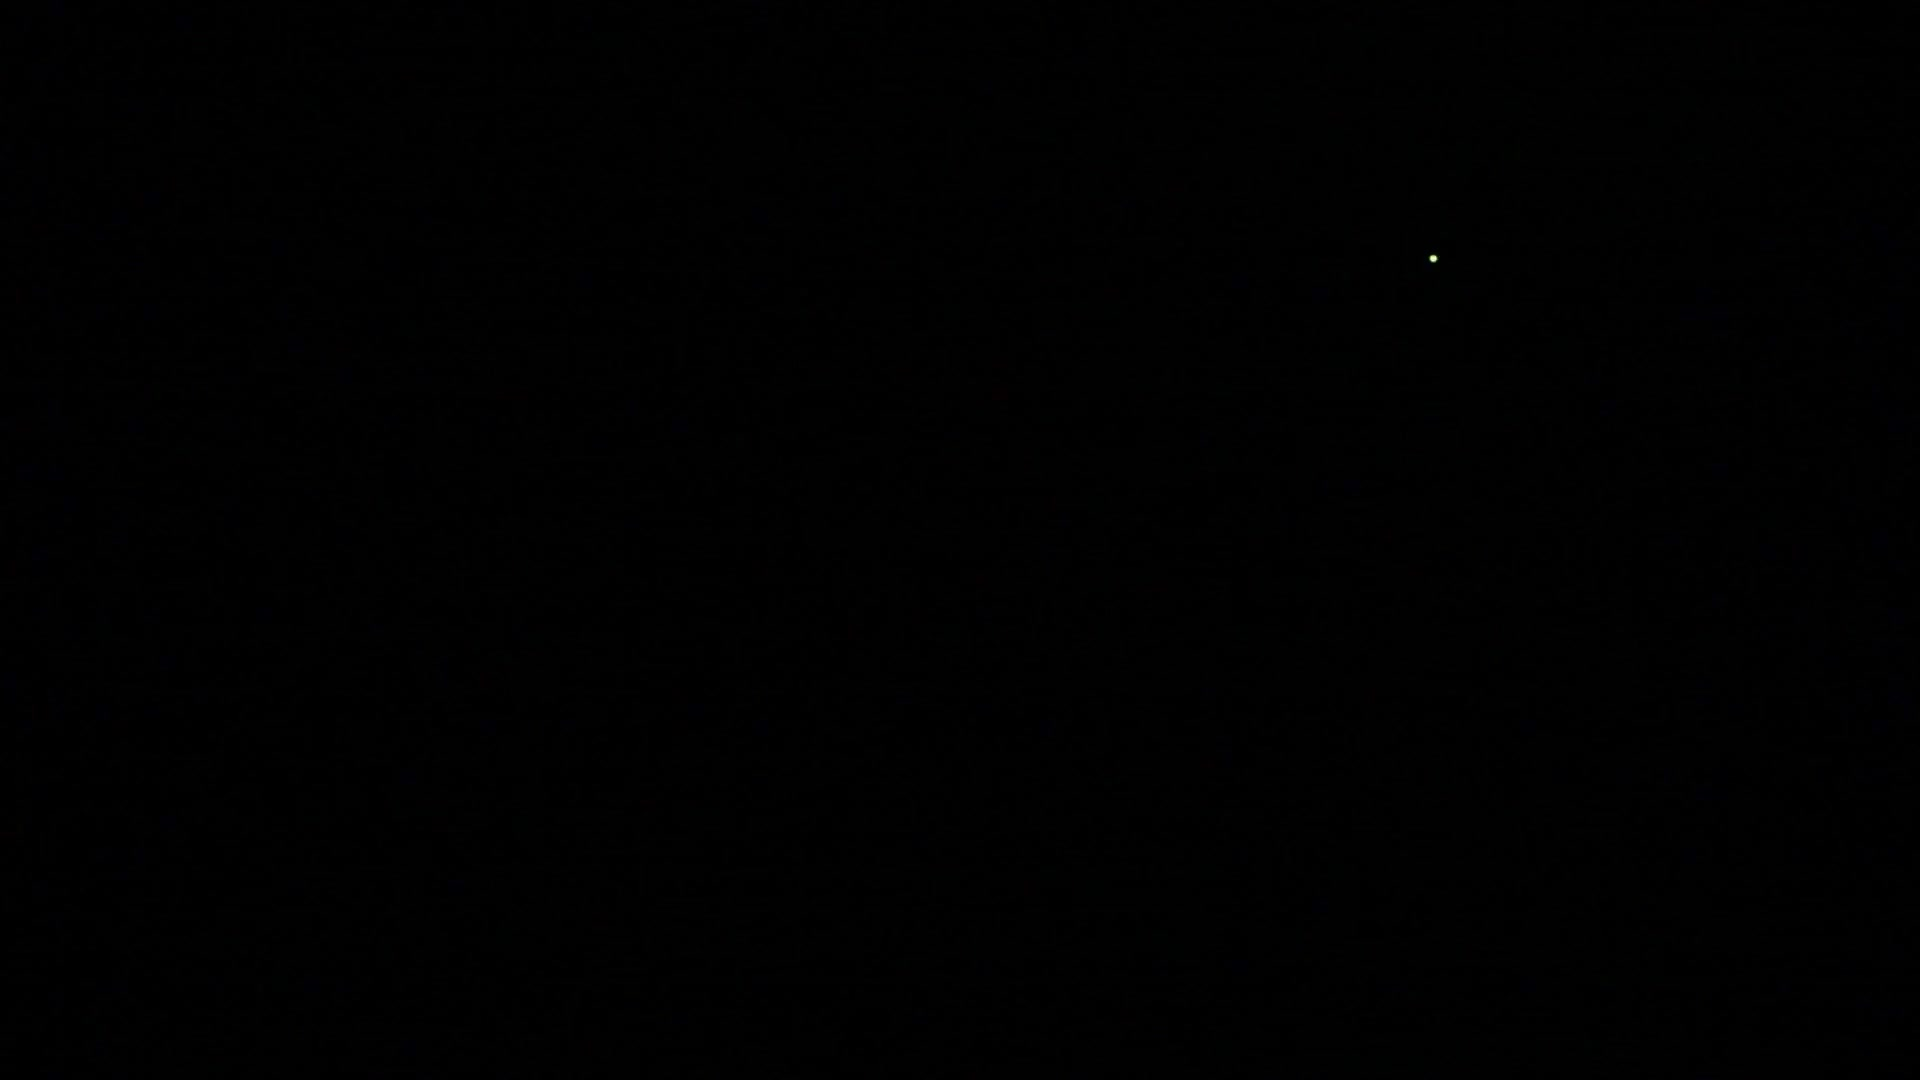
\includegraphics[width=\textwidth]{movies/6006_1}}{movies/6006.mov}
\end{frame}

\end{document}
